\subsubsection{Fixing $a_L = a_R = b_L = 1, c_R = 2.3$}

To better mimic the behavior of the original model function, we now fix the parameters $a_L, a_R, b_L,$ and $c_R$.
Fixing $a_L$ and $b_L$ and varying $c_L$ in the range $[0.8, 1.4]$ will cause the branches $\A$ and $\C$ to move upwards, just as we observed in the original model in \Cref{sec:og.param.effects}.
To get the left part of branches $\B$ and $\D$ to move downwards while also moving the local minima of those branches to the lower left, we vary $b_R$ in the range $[0, 2]$.
\Cref{fig:quadratic.full.cLbR.2d.full} shows a 2D scan of the periods in this model.


\begin{figure}
    \centering
    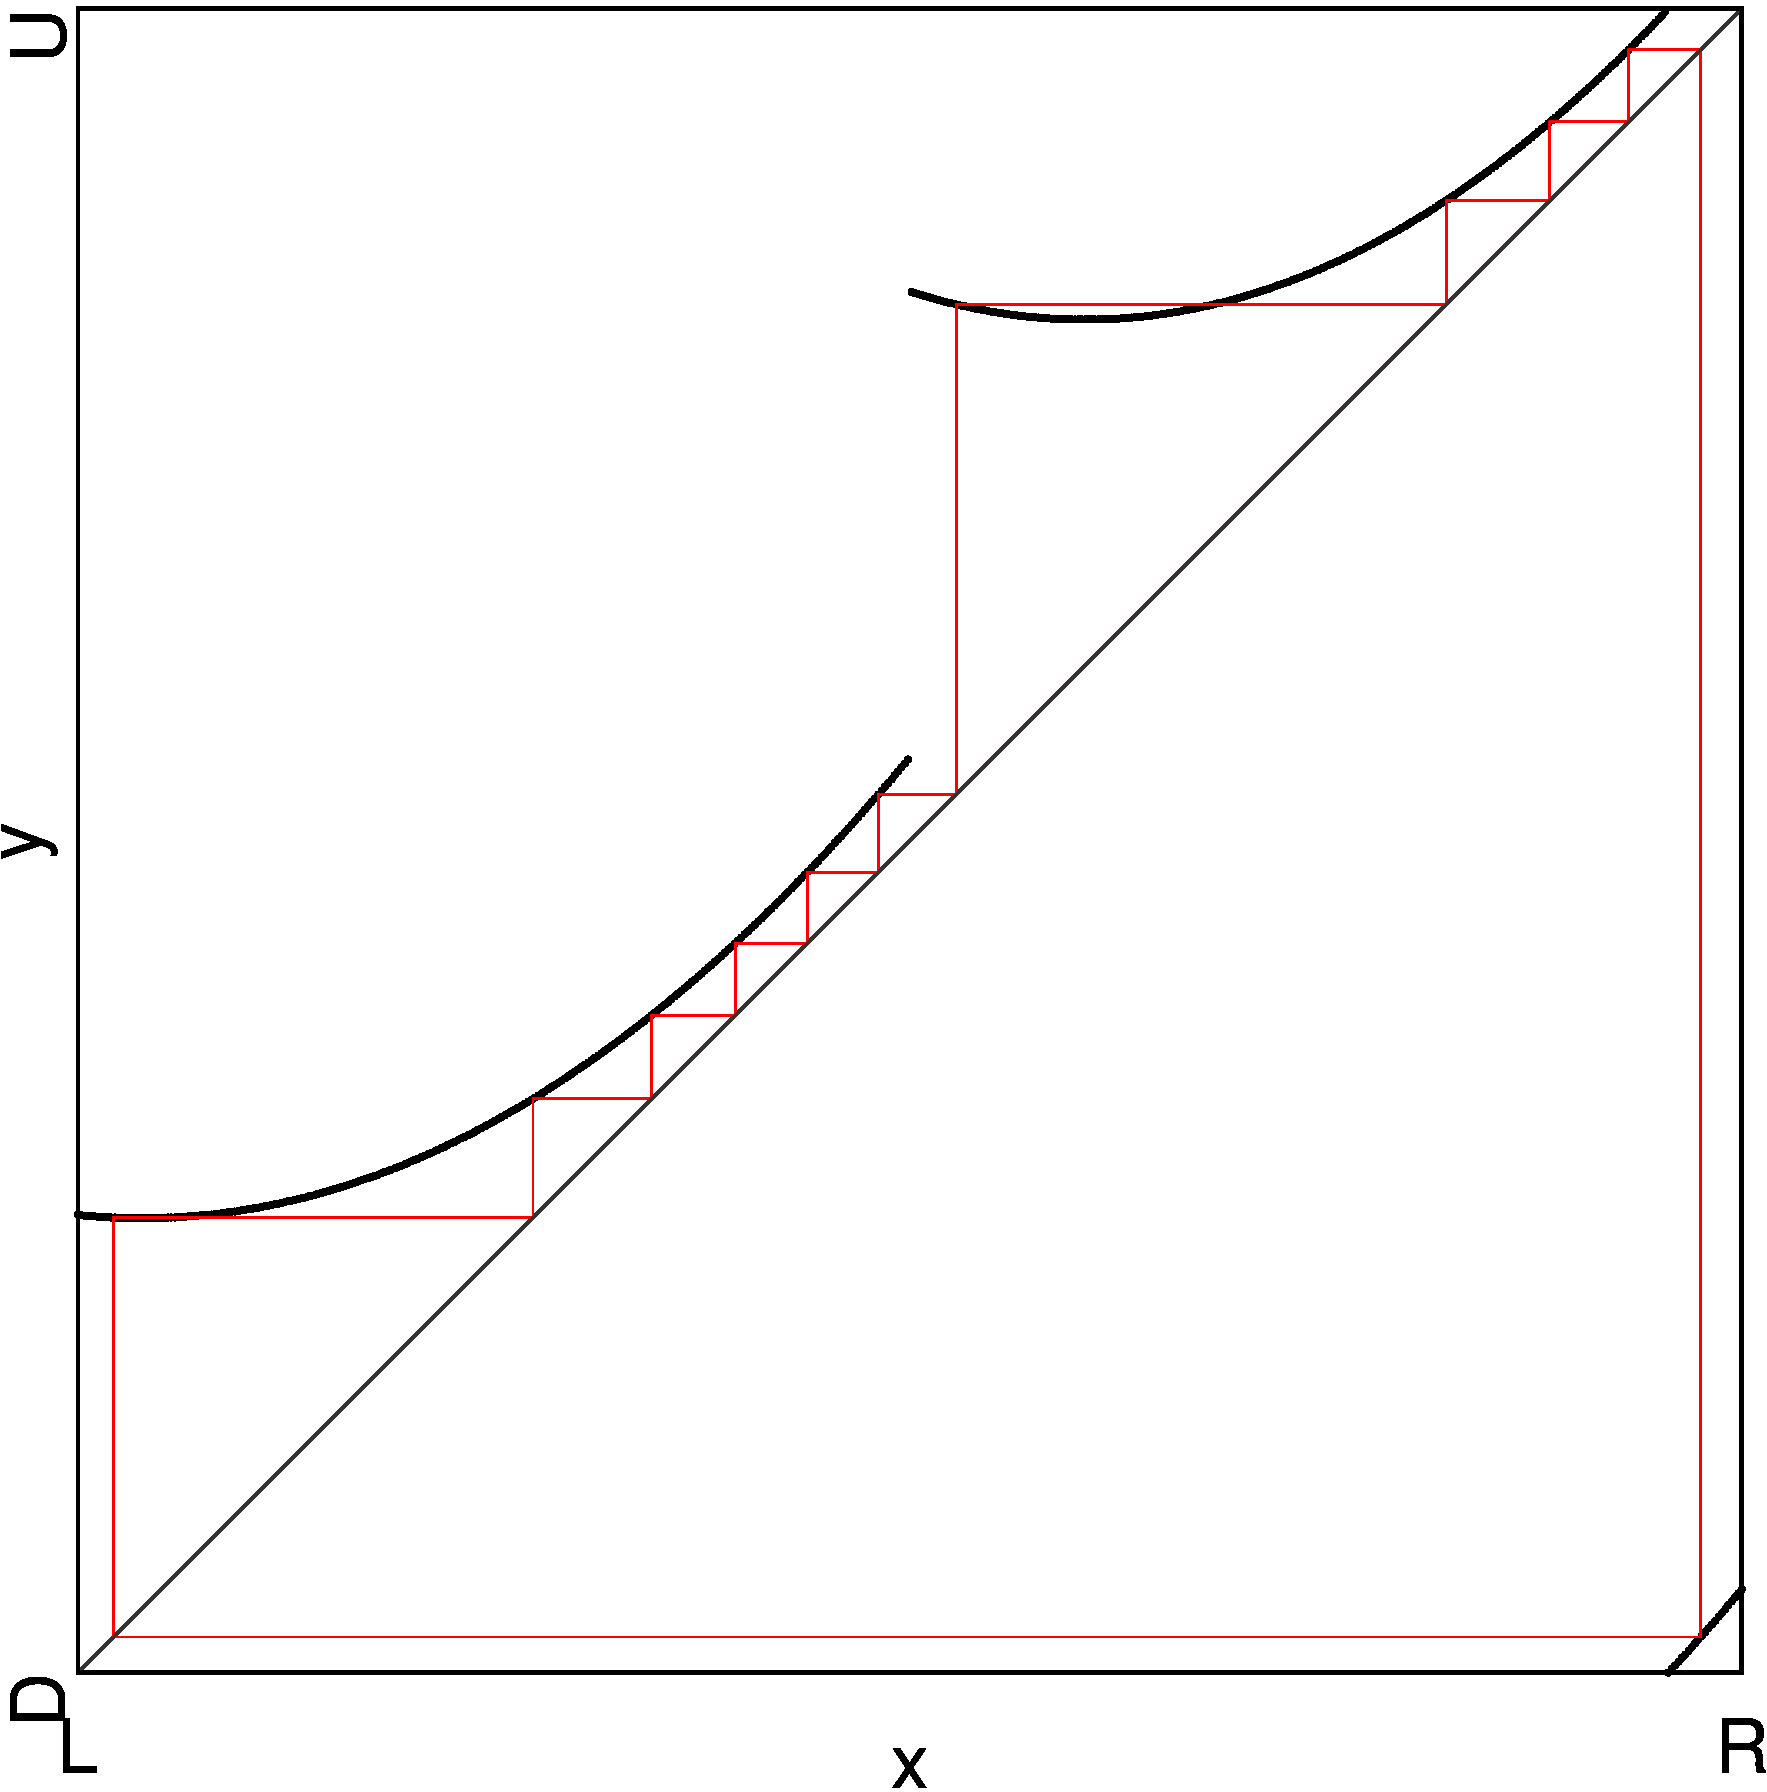
\includegraphics[width=0.6\textwidth]{21_Quadratic_mod6/TestingDifferentParameters/2D_Period_cLbR_Lower/result.png}
    \caption{2D Scan of Quadratic Model Imitating the Original Model}
    \label{fig:quadratic.full.cLbR.2d.full}
\end{figure}

\Cref{fig:quad.full.cLbR.Cobwebs} shows cobwebs along the red line in \Cref{fig:quadratic.full.cLbR.2d.full}.
You can see, that the 14-cycle that existed at the beginning in \Cref{fig:quad.full.cLbR.CobwebA} with symbolic sequence $\A^3\B^4\C^3\D^4$ still exists at the end in \Cref{fig:quad.full.cLbR.CobwebC}.
In \Cref{fig:quad.full.cLbR.CobwebB} you can also see another 14-cycle coexisting.
It has the symbolic sequence $\A^2\B^5\C^2\D^5$.
This is different from the phenomenon, we are searching for.
The reason for this coexistence is, that the arm of the wing crosses this area of period 14.
You can see the arm above the right end of the red line passing through the arm of the area we are examining.

\begin{figure}
    \centering
    \begin{subfigure}{0.3\textwidth}
        \centering
        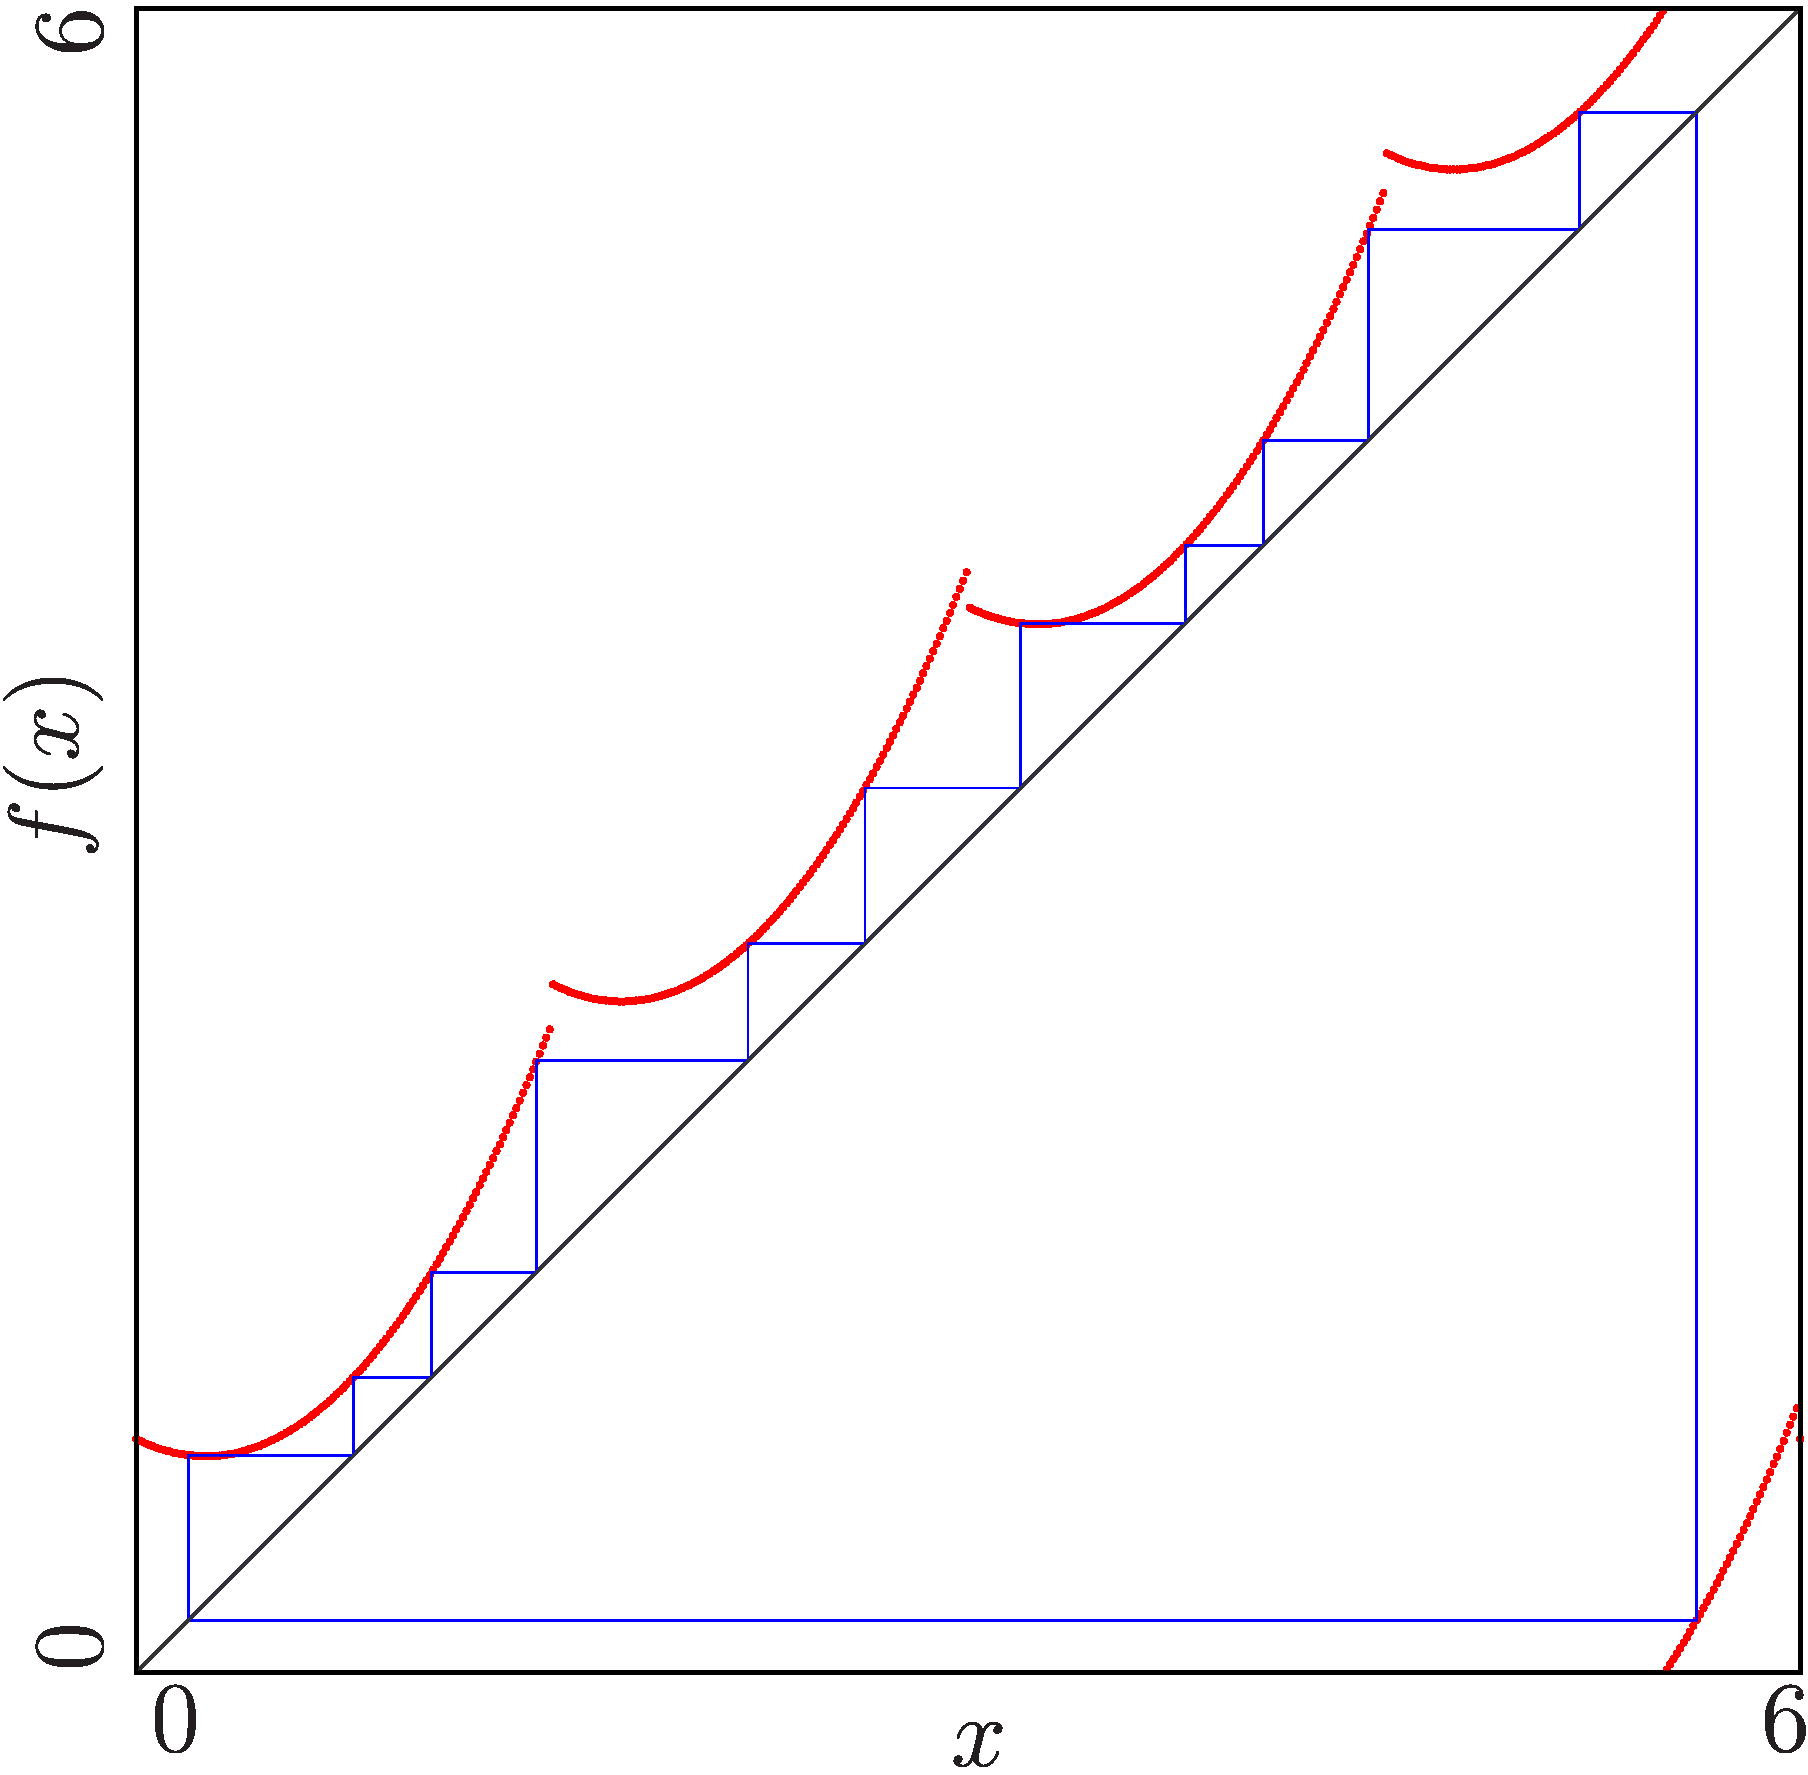
\includegraphics[width=\textwidth]{21_Quadratic_mod6/TestingDifferentParameters/Cobweb_cLbR/result_A.png}
        \caption{Before border}
        \label{fig:quad.full.cLbR.CobwebA}
    \end{subfigure}
    \begin{subfigure}{0.3\textwidth}
        \centering
        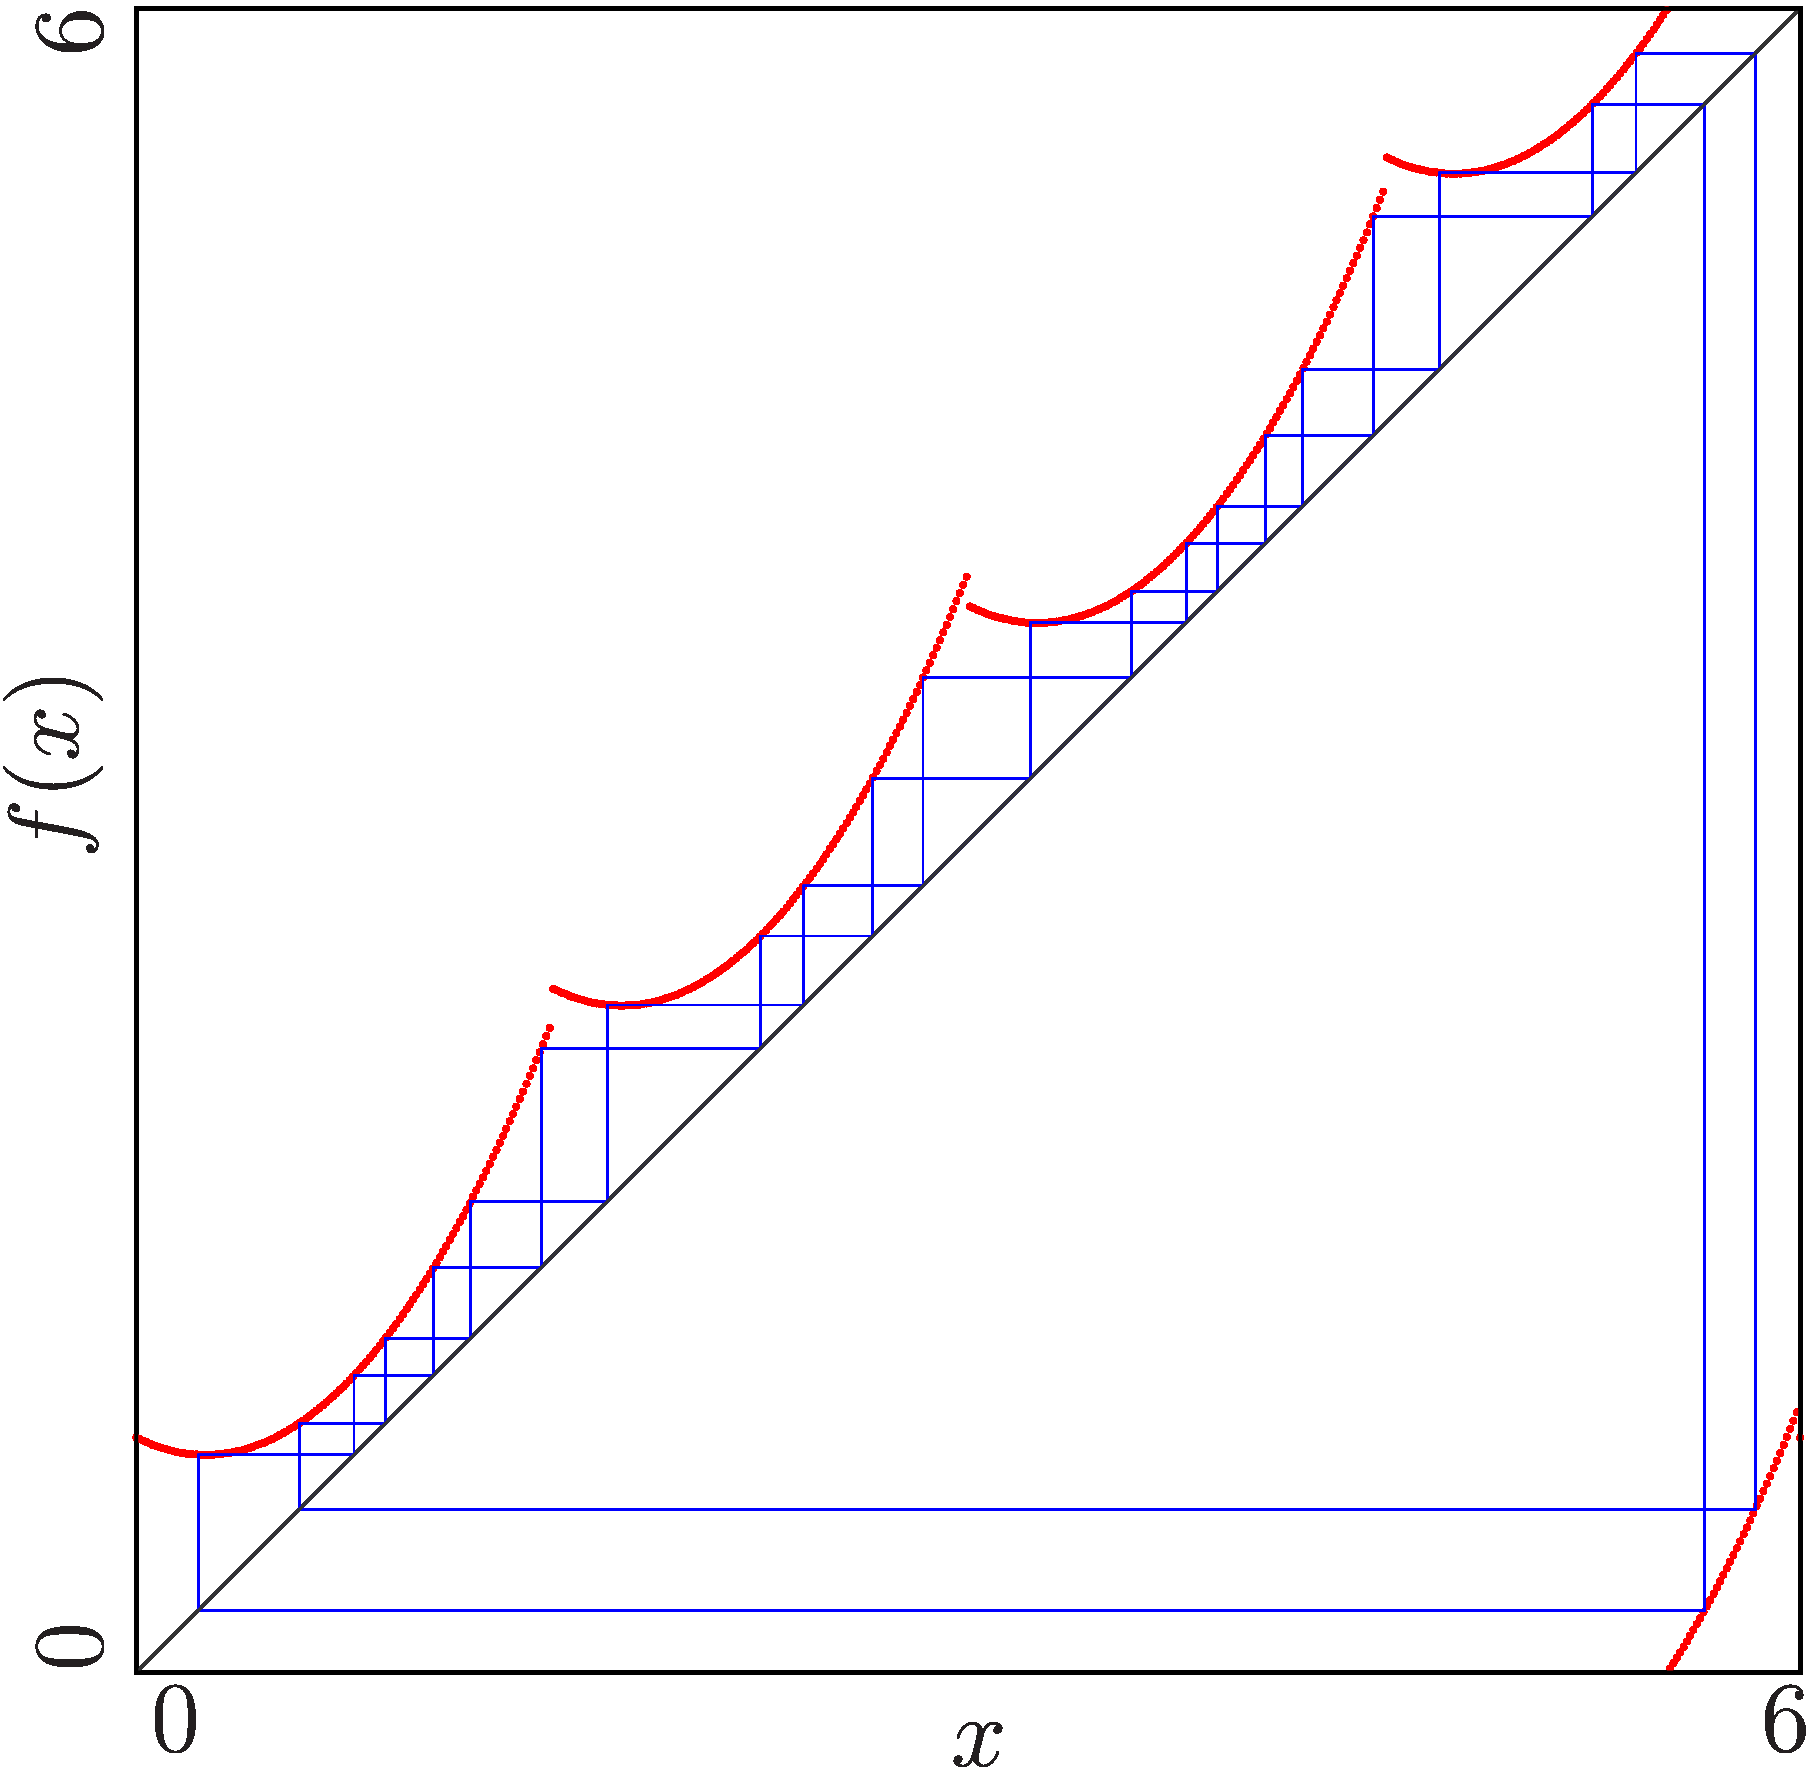
\includegraphics[width=\textwidth]{21_Quadratic_mod6/TestingDifferentParameters/Cobweb_cLbR/result_B.png}
        \caption{At border}
        \label{fig:quad.full.cLbR.CobwebB}
    \end{subfigure}
    \begin{subfigure}{0.3\textwidth}
        \centering
        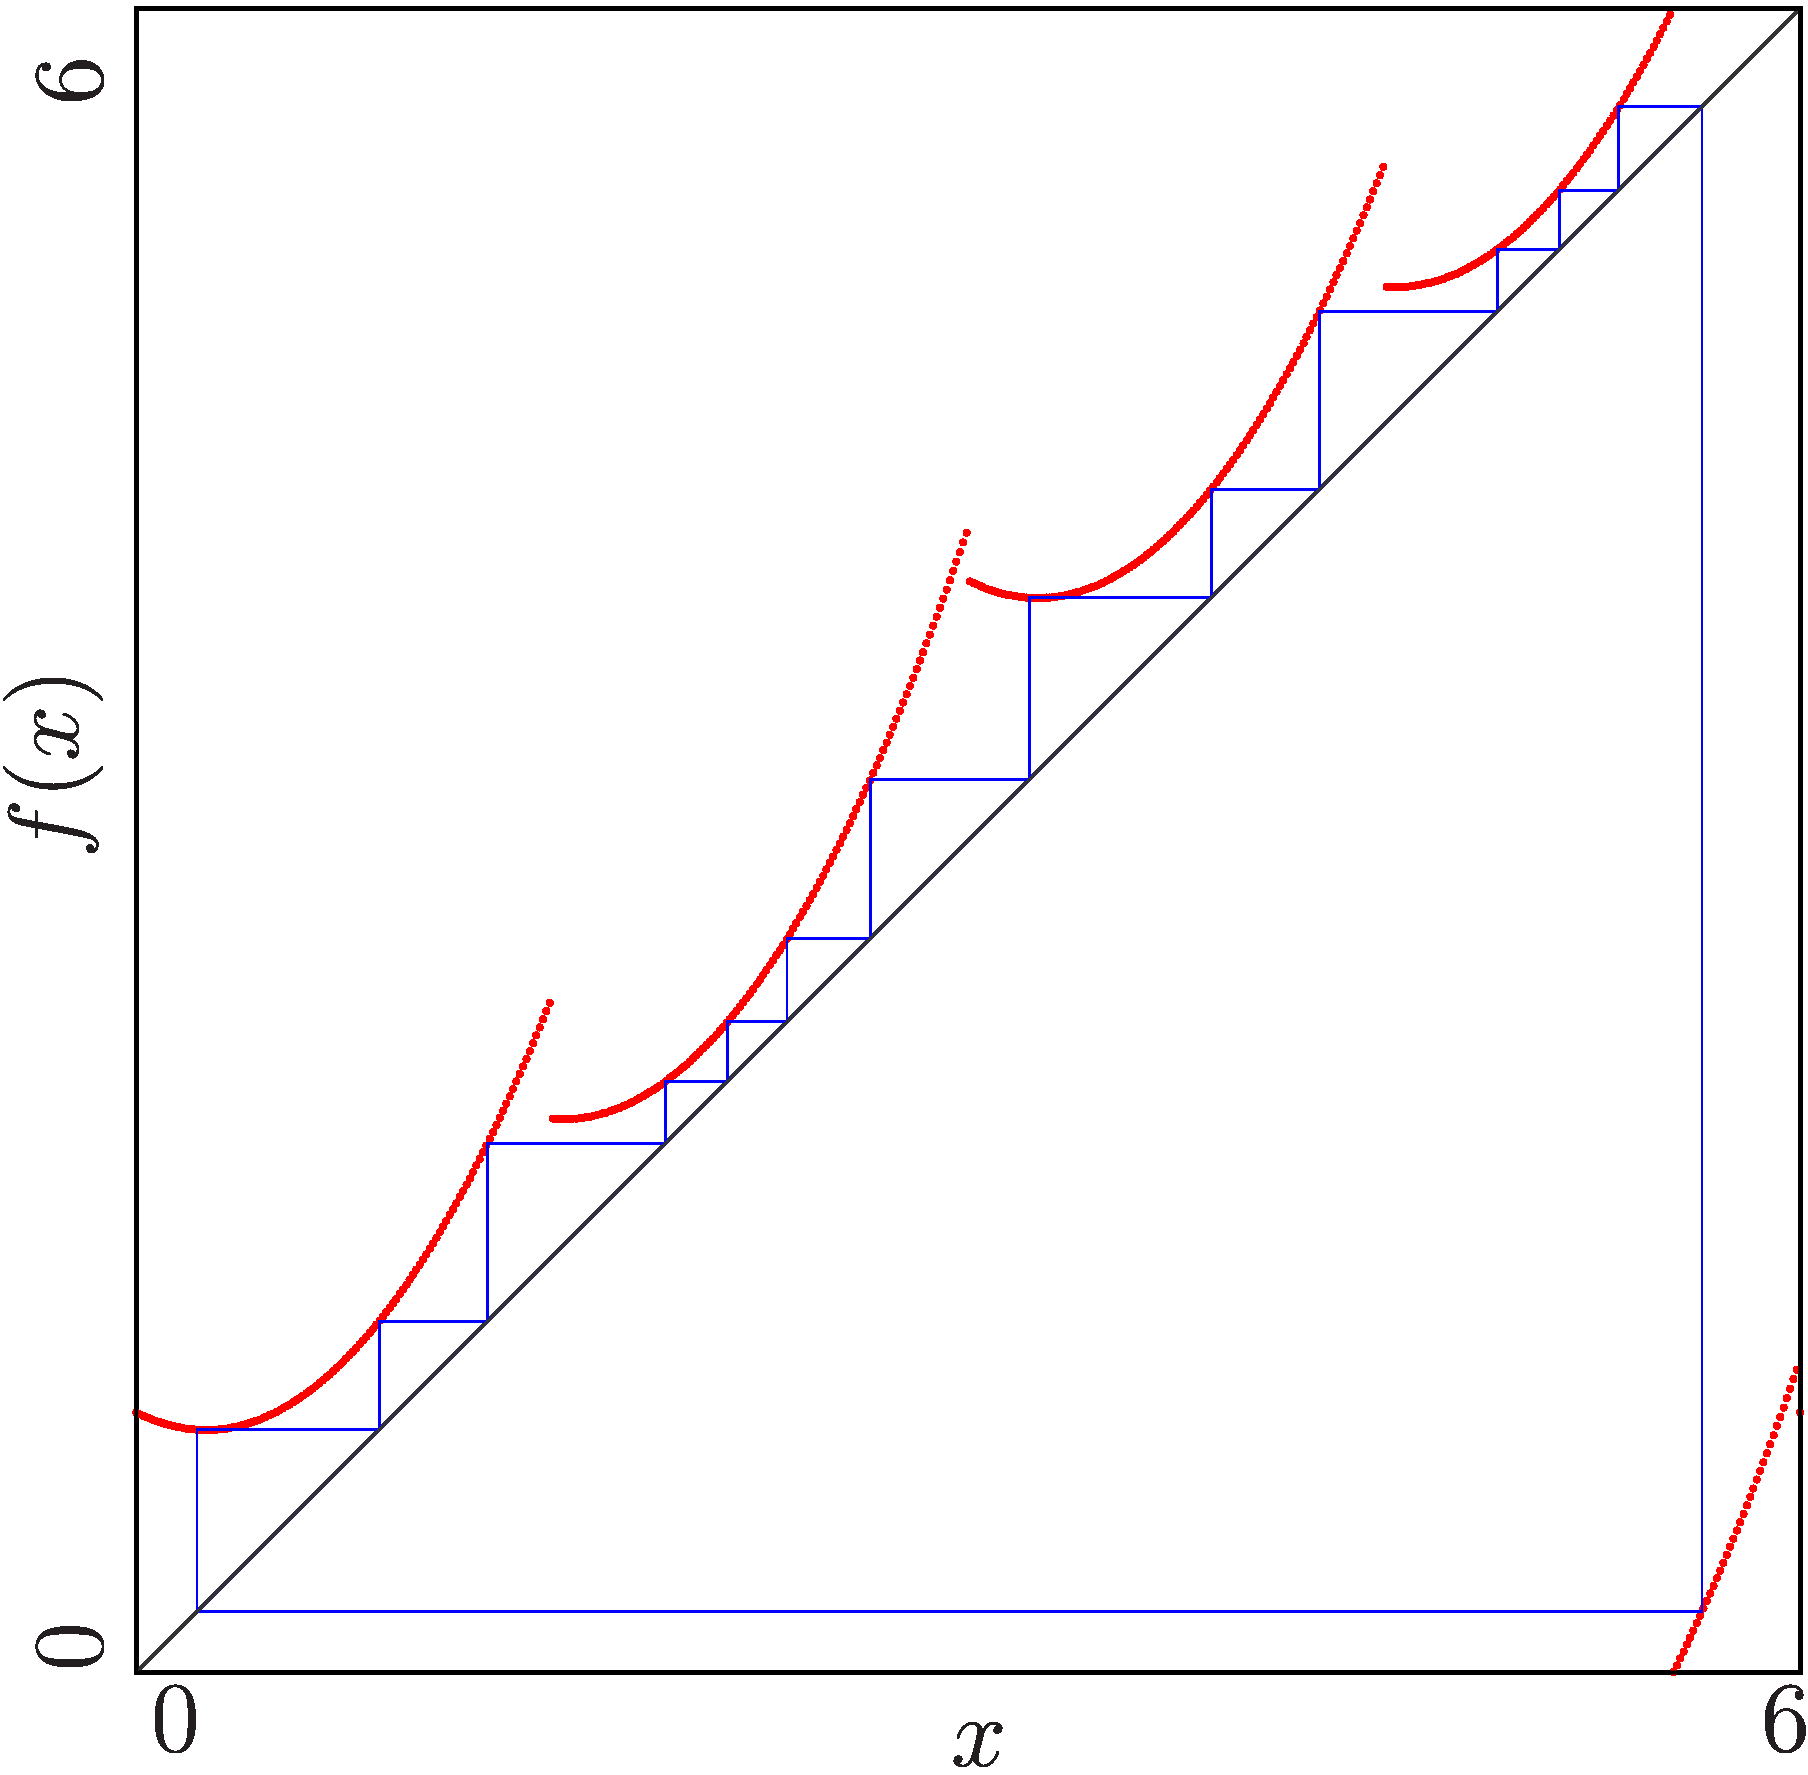
\includegraphics[width=\textwidth]{21_Quadratic_mod6/TestingDifferentParameters/Cobweb_cLbR/result_C.png}
        \caption{After border}
        \label{fig:quad.full.cLbR.CobwebC}
    \end{subfigure}
    \caption{Cobwebs along marked line}
    \label{fig:quad.full.cLbR.Cobwebs}
\end{figure}
